\documentclass[letterpaper,12pt]{article}
\usepackage[utf8]{inputenc}
\usepackage[spanish,es-noquoting]{babel}
\usepackage[T1]{fontenc}
\usepackage{geometry}
\usepackage{graphicx}
\usepackage{enumitem}
\usepackage{color}
\usepackage{tabularx}
\usepackage{float}
\usepackage{caption}
\usepackage{amsmath}
\graphicspath{{img/}}

% Configuración de márgenes
\geometry{
    left=2.5cm,
    right=2.5cm,
    top=2.5cm,
    bottom=2.5cm
}

\definecolor{solcolor}{rgb}{0.0, 0.4, 0.0} % Verde oscuro para distinguir las respuestas

\begin{document}

%%%%%% ENCABEZADO %%%%%%%

\noindent \textbf{Universidad Central de Venezuela}\\
\textbf{Facultad de Ciencias}\\
\textbf{Escuela de Computación}\\
\textbf{Organización y Estructura del Computador II}\\
Semestre 01-2026

\vspace{0.3cm}
\begin{center}
{\textbf{Respuestas - Práctica: Microarquitectura}}
\end{center}
\vspace{0.5cm}

%%%%%% CONTENIDO %%%%%%%

\begin{enumerate}

    %%%%% PREGUNTA 1 %%%%%
    \item Se desea rediseñar una de las unidades del procesador RISC-V de ciclo único para que tenga la mitad del retraso. Usando los retrasos de la siguiente tabla, responda lo siguiente:

    \begin{center}
        \small
        \begin{tabular}{|l|c|r|}
            \hline
            \textbf{Element} & \textbf{Parameter} & \textbf{Delay (ps)} \\
            \hline
            Register clk-to-Q & $t_{pcq}$ & 40 \\
            Register setup & $t_{setup}$ & 50 \\
            Multiplexer & $t_{mux}$ & 30 \\
            AND-OR gate & $t_{\text{AND-OR}}$ & 20 \\
            ALU & $t_{\text{ALU}}$ & 120 \\
            Decoder (control unit) & $t_{\text{dec}}$ & 25 \\
            Extend unit & $t_{\text{ext}}$ & 35 \\
            Memory read & $t_{\text{mem}}$ & 200 \\
            Register file read & $t_{\text{RFread}}$ & 100 \\
            Register file setup & $t_{\text{RFsetup}}$ & 60 \\
            \hline
        \end{tabular}
    \end{center}

    \begin{enumerate}[label=\alph*)]
        \item ¿En qué unidad debería trabajar para obtener la mayor aceleración del procesador general?

        {\color{solcolor}
        \textbf{Solución:}
        Para aumentar al máximo el rendimiento (es decir, disminuir el tiempo de ciclo), se debe acelerar la \textbf{unidad de memoria}. Esto se debe a que el tiempo de lectura de memoria tiene un retardo de $200\,\text{ps}$, el cual es estrictamente mayor al de cualquiera de las otras unidades del procesador.
        }

        \vspace{0.3cm}
        \item ¿Cuál sería el tiempo de ciclo de la máquina mejorada? Explique.

        {\color{solcolor}
        \textbf{Solución:}
        Empleando la fórmula de cálculo del tiempo de ciclo para un procesador RISC-V de ciclo único (camino crítico correspondiente a la instrucción \texttt{lw}) y teniendo en cuenta que se tendrá la mitad del retraso para la unidad de memoria ($t_{\text{mem}} = 200/2 = 100\,\text{ps}$), el tiempo de ciclo de la máquina mejorada es:
        \[
        T_{c\_new} = t_{pcq\_PC} + 2t_{\text{mem}} + t_{\text{RFread}} + t_{\text{ALU}} + t_{mux} + t_{\text{RFsetup}}
        \]
        \[
        T_{c\_new} = 40 + 2(100) + 100 + 120 + 30 + 60 = \mathbf{550\text{ ps}}
        \]
        }
    \end{enumerate}

    \vspace{0.6cm}

    %%%%% PREGUNTA 2 %%%%%
    \item Repita el ejercicio 1b para un procesador RISC-V multiciclo.

    {\color{solcolor}
    \textbf{Solución:}
    Para determinar el tiempo de ciclo del procesador multiciclo, empleamos la fórmula:
    \[
    T_{c\_multi} = t_{pcq} + t_{\text{dec}} + 2t_{mux} + \max[t_{\text{ALU}},\, t_{\text{mem}}] + t_{setup}
    \]
    Con la memoria mejorada a la mitad de su retardo ($t_{\text{mem}} = 100\,\text{ps}$):
    \[
    T_{c\_multi\_new} = t_{pcq} + t_{\text{dec}} + 2t_{mux} + \max[t_{\text{ALU}},\, t_{\text{mem}}] + t_{setup}
    \]
    \[
    T_{c\_multi\_new} = 40 + 25 + 2(30) + \max[120,\, 100] + 50
    \]
    \[
    T_{c\_multi\_new} = 40 + 25 + 60 + 120 + 50 = \mathbf{295\text{ ps}}
    \]
    }

    \vspace{0.6cm}

    %%%%% PREGUNTA 3 %%%%%
    \item ¿Cuántos ciclos se requieren para ejecutar el siguiente programa en el procesador multiciclo RISC-V? ¿Cuál es el CPI de este programa?

    \begin{verbatim}
          addi s0, zero, 5      # result = 5
    L1:
          bge  zero, s0, Done   # if result <= 0, exit loop
          addi s0, s0, -1       # result = result - 1
          j    L1
    Done:
    \end{verbatim}

    {\color{solcolor}
    \textbf{Solución:}
    El programa ejecutará 6 instrucciones \texttt{addi} (4 ciclos cada una), 6 \texttt{bge} (3 ciclos cada una) y 5 \texttt{jal} (4 ciclos cada una) para un total de:
    \[
    (6 \times 4) + (6 \times 3) + (5 \times 4) = 24 + 18 + 20 = \mathbf{62\text{ ciclos de reloj para 17 instrucciones.}}
    \]
    Así, el CPI de este programa es:
    \[
    \text{CPI} = \frac{62}{17} \approx \mathbf{3{,}65\text{ CPI}}
    \]
    \textit{(Recuerde que \texttt{j L1} es una pseudoinstrucción para \texttt{jal x0, L1})}.
    }

    \vspace{0.6cm}

    \pagebreak

    %%%%% PREGUNTA 4 %%%%%
    \item El procesador RISC-V segmentado (\textit{pipelined RISC-V}) ejecuta el siguiente fragmento de código. ¿Qué registros se escriben y cuáles se leen en el quinto ciclo? Recuerde que el procesador RISC-V segmentado tiene una unidad de riesgo. Puede asumir un sistema de memoria que devuelve el resultado dentro de un ciclo.

    \begin{verbatim}
    addi s1, zero, 52   # s1 = 52
    addi s0, s1, -4     # s0 = s1 - 4 = 48
    lw   s3, 16(s0)     # s3 = memory[64]
    sw   s3, 20(s0)     # memory[68] = s3
    xor  s2, s0, s3     # s2 = s0 ^ s3
    or   s2, s2, s3     # s2 = s2 | s3
    \end{verbatim}

    {\color{solcolor}
    \textbf{Solución:}

    El código se ejecuta a través de las etapas del cauce (\textit{Pipeline stages}) de acuerdo a la siguiente tabla:

    \begin{center}
        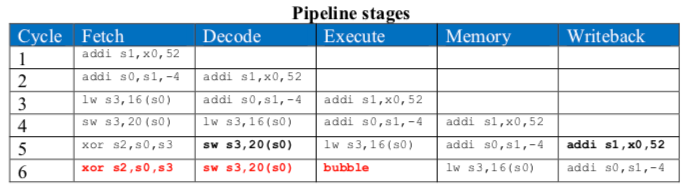
\includegraphics[width=0.92\linewidth]{tabla_pipeline_ciclos.png}
    \end{center}

    En el \textbf{ciclo 5}:
    \begin{itemize}
        \item El registro \textbf{\texttt{s1}} está siendo \textbf{escrito} (por la primera instrucción \texttt{addi}) en la etapa de decodificación (\textit{Decode} / etapa donde el banco de registros se escribe en la primera mitad del ciclo o en \textit{Writeback}).
        \item Los registros \textbf{\texttt{s0}} y \textbf{\texttt{s3}} están siendo \textbf{leídos} por la instrucción \texttt{sw} en la etapa de decodificación (\textit{Decode}).
    \end{itemize}
    Tenga en cuenta que, en este ciclo, \texttt{sw} detecta que necesita detenerse (\textit{stall}) en el siguiente ciclo, porque un \texttt{lw} está en la etapa de ejecución (\textit{Execute}) que producirá uno de sus registros de origen (\texttt{s3}), y el \texttt{lw} no tendrá ese operando listo hasta el final de la etapa de Memoria.
    }

    \vspace{0.6cm}

    \pagebreak

    %%%%% PREGUNTA 5 %%%%%
    \item Usando un diagrama de pipeline similar al visto en clase, muestre el adelanto y las paradas necesarias para ejecutar las instrucciones del ejercicio 4 en el procesador RISC-V segmentado.

    {\color{solcolor}
    \textbf{Solución:}

    A continuación se muestra el diagrama de pipeline con las líneas de adelanto (\textit{forwarding}) y la parada (\textit{stall}):

    \begin{center}
        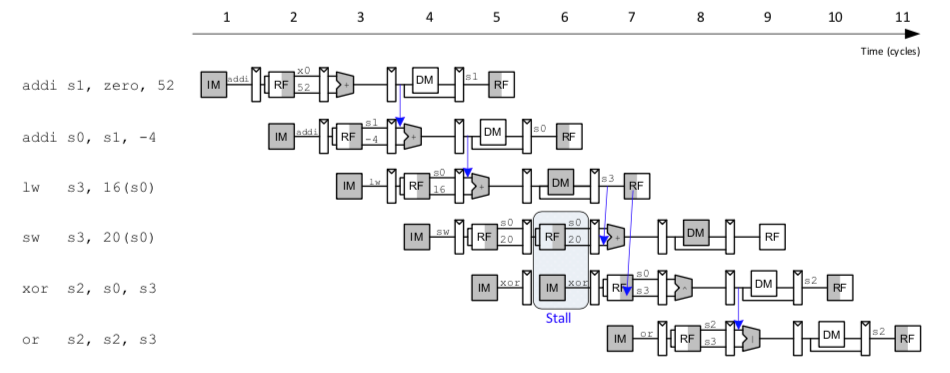
\includegraphics[width=\linewidth]{diagrama_adelanto_paradas.png}
    \end{center}
    }

    \vspace{0.6cm}

    %%%%% PREGUNTA 6 %%%%%
    \item ¿Cuántos ciclos se requieren para que el procesador RISC-V segmentado emita todas las instrucciones para el programa del ejercicio 4? ¿Cuál es el CPI del procesador en este programa?

    {\color{solcolor}
    \textbf{Solución:}

    Se necesitan \textbf{7 ciclos de reloj} para emitir todas las instrucciones (hasta que la sexta instrucción entra a la etapa \textit{Fetch}).

    \[
    \#\text{ instrucciones} = 6
    \]
    \[
    \text{CPI} = \frac{7\text{ ciclos de reloj}}{6\text{ instrucciones}} \approx \mathbf{1{,}17\text{ CPI}}
    \]
    }

    \vspace{0.6cm}

    \pagebreak

    %%%%% PREGUNTA 7 %%%%%
    \item Se desea que ud rediseñe una de las unidades del procesador RISC-V segmentado para que sea mucho más rápido. Usando los retrasos de la tabla del ejercicio 1, responda ¿en qué unidad debería trabajar para obtener la mayor aceleración del procesador general? ¿Cuánto más rápido podrá ser? ¿Cuál es el tiempo de ciclo del procesador mejorado? Explique tus respuestas.

    {\color{solcolor}
    \textbf{Solución:}

    Ecuación del ciclo de reloj para el procesador segmentado:
    \[
    T_{c\_\text{pipelined}} = \max
    \left[
    \begin{array}{ll}
        t_{pcq} + t_{\text{mem}} + t_{setup} & \text{Fetch} \\
        2(t_{\text{RFread}} + t_{setup}) & \text{Decode} \\
        t_{pcq} + 4t_{mux} + t_{\text{ALU}} + t_{\text{AND-OR}} + t_{setup} & \text{Execute} \\
        t_{pcq} + t_{\text{mem}} + t_{setup} & \text{Memory} \\
        2(t_{pcq} + t_{mux} + t_{\text{RFsetup}}) & \text{Writeback}
    \end{array}
    \right]
    \]

    Sustituyendo los valores de retardo:
    \[
    T_{c3} = \max
    \left[
    \begin{array}{l}
        40 + 200 + 50 \\
        2(100 + 50) \\
        40 + 4(30) + 120 + 20 + 50 \\
        40 + 200 + 50 \\
        2(40 + 30 + 60)
    \end{array}
    \right]
    = \max [290,\, 300,\, 350,\, 290,\, 260] = \mathbf{350\text{ ps}}
    \]

    \textbf{Analizando:}
    \begin{itemize}
        \item La etapa más lenta es la \textbf{etapa de ejecución (\textit{Execute})} con $350\,\text{ps}$.
        \item La siguiente etapa más lenta es la \textbf{etapa de decodificación (\textit{Decode})} con $300\,\text{ps}$.
        \item La etapa de ejecución debe reducirse en $50\,\text{ps}$ para que sea tan rápida como la etapa de decodificación.
        \item Debería, en consecuencia, reducirse el retraso de la \textbf{ALU} a:
        \[
        t_{\text{ALU\_nuevo}} = 120 - 50 = \mathbf{70\text{ ps}}
        \]
    \end{itemize}
    El nuevo tiempo de ciclo es \textbf{300 ps}.
    }

\end{enumerate}

\end{document}
